\chapter{Evaluation}

\begin{figure}[hbtp]
	\centering
	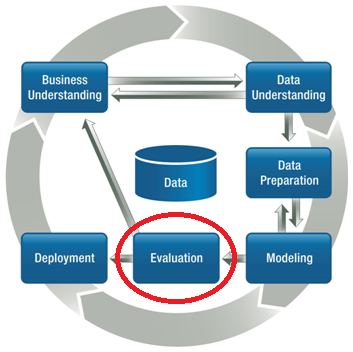
\includegraphics[width=0.5\textwidth]{./images/CRISPDM_5.png}
	\caption{CRISP-DM - Evaluation}
	\label{CRISPDM_5}
\end{figure}
In questa fase si andranno a valutare i risultati ottenuti dall'intero processo CRISP-DM fatto finora. Se tale valutazione risulta essere non positiva rispetto a ciò che il sistema si prefiggeva di fare, si passerà alla definizione di altri parametri o alla scelta di altri tipi di algoritmi per effettuare la classificazione.
\pagebreak
\section{Valutazione rispetto agli obiettivi di business}
I risultati ottenuti, mostrati nello schema \ref{Risultati}, possono essere considerati positivi rispetto agli obiettivi di business, in quanto supera il 99 \% di correttezza richiesto dal task \ref{task}. 
Tuttavia, al fine di tentare di migliorare ulteriormente il sistema di classificazione, sono state testate le varianti che il modello FT offriva (\emph{Alberi funzionali ai soli nodi intermedi} \ref{Alberi funzionali ai soli nodi intermedi} e \emph{Alberi funzionali ai soli nodi foglia} \ref{Alberi funzionali ai soli nodi foglia}). Per fare ciò, è stato necessario variare il parametro modelType rispettivamente in \emph{FT Inner} e \emph{FT Leaves}.

Inoltre, per completezza, è stato fatto un esperimento controllato avente 3 fattori con n livelli:
%sono state sperimentate altre configurazioni sul dataset combinando tutti gli algoritmi definiti finora :

%\begin{multicols}{3}
%\textbf{Sampling}:
%\begin{itemize}
%	\item con SMOTE
%	\item senza SMOTE
%\end{itemize}
%\columnbreak
%
%\textbf{Feature Selection}:
%\begin{itemize}
%	\item con CfsSubsetEval
%	\item senza CfsSubsetEval
%\end{itemize}
%
%\columnbreak
%
%\textbf{Classifiers}:
%\begin{itemize}
%	\item FT
%	\item FT-Leaves
%	\item FT-Inner
%\end{itemize}
%\end{multicols}
\vspace{0.5cm}
\textbf{Sampling}:
\begin{itemize}
	\item con SMOTE
	\item senza SMOTE
\end{itemize}
\vspace{0.5cm}
\textbf{Feature Selection}:
\begin{itemize}
	\item con CfsSubsetEval
	\item senza CfsSubsetEval
\end{itemize}
\vspace{0.5cm}
\textbf{Classifiers}:
\begin{itemize}
	\item FT
	\item FT-Leaves
	\item FT-Inner
\end{itemize}

Di seguito verranno riportati i risultati ottenuti da queste configurazioni.
\pagebreak 
\subsection{Risultati Configurazioni}
\paragraph{FT - Original Dataset}
{\scriptsize
	\begin{verbatim}
		=== Stratified cross-validation ===
		=== Summary ===
		
		Correctly Classified Instances        7910               98.875  %
		Incorrectly Classified Instances        90                1.125  %
		Kappa statistic                          0.9763
		Mean absolute error                      0.0139
		Root mean squared error                  0.1001
		Relative absolute error                  2.9227 %
		Root relative squared error             20.5236 %
		Total Number of Instances             8000     
		
		=== Detailed Accuracy By Class ===
		
		       TP Rate   FP Rate   Precision   Recall  F-Measure   ROC Area  Class
		        0.984     0.008      0.987     0.984     0.986      0.994    yes
		        0.992     0.016      0.99      0.992     0.991      0.994    no
		Mean    0.989     0.013      0.989     0.989     0.989      0.994
		
		=== Confusion Matrix ===
		
		  a     b   <-- classified as
		3063   49 |      a = yes
		41   4847 |      b = no
	\end{verbatim}
}

\paragraph{FT - CfsSubsetEval}
{\scriptsize
	\begin{verbatim}
	=== Stratified cross-validation ===
	=== Summary ===
	
	Correctly Classified Instances        7898               98.725  %
	Incorrectly Classified Instances       102                1.275  %
	Kappa statistic                          0.9731
	Mean absolute error                      0.0164
	Root mean squared error                  0.1072
	Relative absolute error                  3.4493 %
	Root relative squared error             21.996  %
	Total Number of Instances             8000     
	
	=== Detailed Accuracy By Class ===
	
	        TP Rate   FP Rate   Precision   Recall  F-Measure   ROC Area  Class
	        0.979     0.007      0.988     0.979     0.984      0.99     yes
	        0.993     0.021      0.987     0.993     0.99       0.99     no
	Mean    0.987     0.016      0.987     0.987     0.987      0.99 
	
	=== Confusion Matrix ===
	
	  a     b   <-- classified as
	3046   66   |    a = yes
	36     4852 |    b = no
	\end{verbatim}
}

\pagebreak
\paragraph{FT - SMOTE}
{\scriptsize
	\begin{verbatim}
	=== Stratified cross-validation ===
	=== Summary ===
	
	Correctly Classified Instances       10992               98.9201 %
	Incorrectly Classified Instances       120                1.0799 %
	Kappa statistic                          0.9781
	Mean absolute error                      0.0121
	Root mean squared error                  0.0972
	Relative absolute error                  2.4639 %
	Root relative squared error             19.5852 %
	Total Number of Instances            11112     
	
	=== Detailed Accuracy By Class ===
	
	       TP Rate   FP Rate   Precision   Recall  F-Measure   ROC Area  Class
	        0.99      0.012      0.99      0.99      0.99       0.995    yes
	        0.988     0.01       0.988     0.988     0.988      0.995    no
	Mean    0.989     0.011      0.989     0.989     0.989      0.995
	
	=== Confusion Matrix ===
	
	  a     b   <-- classified as
	6164   60 |    a = yes
	60   4828 |    b = no
	\end{verbatim}
}

\paragraph{FT Inner - Original}
{\scriptsize
	\begin{verbatim}
	=== Stratified cross-validation ===
	=== Summary ===
	
	Correctly Classified Instances        7908               98.85   %
	Incorrectly Classified Instances        92                1.15   %
	Kappa statistic                          0.9758
	Mean absolute error                      0.0115
	Root mean squared error                  0.1072
	Relative absolute error                  2.4192 %
	Root relative squared error             21.9965 %
	Total Number of Instances             8000     
	
	=== Detailed Accuracy By Class ===
	
	        TP Rate   FP Rate   Precision   Recall  F-Measure   ROC Area  Class
	        0.985     0.009      0.986     0.985     0.985      0.988    yes
	        0.991     0.015      0.99      0.991     0.991      0.988    no
	Mean    0.989     0.013      0.988     0.989     0.988      0.988
	
	=== Confusion Matrix ===
	
	 a      b   <-- classified as
	3064   48   |      a = yes
	44     4844 |      b = no
	\end{verbatim}
}

\pagebreak
\paragraph{FT Inner - CfsSubsetEval}
{\scriptsize
	\begin{verbatim}
	=== Stratified cross-validation ===
	=== Summary ===
	
	Correctly Classified Instances        7896               98.7    %
	Incorrectly Classified Instances       104                1.3    %
	Kappa statistic                          0.9726
	Mean absolute error                      0.013 
	Root mean squared error                  0.114 
	Relative absolute error                  2.7347 %
	Root relative squared error             23.3871 %
	Total Number of Instances             8000     
	
	=== Detailed Accuracy By Class ===
	
	       TP Rate   FP Rate   Precision   Recall  F-Measure   ROC Area  Class
	        0.978     0.007      0.988     0.978     0.983      0.985    yes
	        0.993     0.022      0.986     0.993     0.989      0.985    no
	Mean    0.987     0.016      0.987     0.987     0.987      0.985
	
	=== Confusion Matrix ===
	
	  a     b   <-- classified as
	3044   68   |    a = yes
	36     4852 |    b = no	
	\end{verbatim}
}

\paragraph{FT Inner - SMOTE}
{\scriptsize
	\begin{verbatim}
	=== Stratified cross-validation ===
	=== Summary ===
	
	Correctly Classified Instances       10985               98.8571 %
	Incorrectly Classified Instances       127                1.1429 %
	Kappa statistic                          0.9768
	Mean absolute error                      0.0114
	Root mean squared error                  0.1069
	Relative absolute error                  2.3193 %
	Root relative squared error             21.5376 %
	Total Number of Instances            11112     
	
	=== Detailed Accuracy By Class ===
	
	       TP Rate   FP Rate   Precision   Recall  F-Measure   ROC Area  Class
	        0.991     0.014      0.989     0.991     0.99       0.988    yes
	        0.986     0.009      0.988     0.986     0.987      0.988    no
	Mean    0.989     0.012      0.989     0.989     0.989      0.988
	
	=== Confusion Matrix ===
	
	  a     b   <-- classified as
	6165   59   |    a = yes
	68     4820 |    b = no	
	\end{verbatim}
}

\pagebreak
\paragraph{FT Inner - SMOTE - CfsSubsetEval}
{\scriptsize
	\begin{verbatim}
	=== Stratified cross-validation ===
	=== Summary ===
	
	Correctly Classified Instances       11001               99.0011 %
	Incorrectly Classified Instances       111                0.9989 %
	Kappa statistic                          0.9797
	Mean absolute error                      0.01  
	Root mean squared error                  0.0999
	Relative absolute error                  2.0271 %
	Root relative squared error             20.1353 %
	Total Number of Instances            11112     
	
	=== Detailed Accuracy By Class ===
	
	       TP Rate   FP Rate   Precision   Recall  F-Measure   ROC Area  Class
	        0.988     0.008      0.994     0.988     0.991      0.99     yes
	        0.992     0.012      0.985     0.992     0.989      0.99     no
	Mean    0.99      0.009      0.99      0.99      0.99       0.99 
	
	=== Confusion Matrix ===
	
	  a     b   <-- classified as
	6150   74   |    a = yes
	37     4851 |    b = no
	\end{verbatim}
}

\paragraph{FT Leaves - Original}
{\scriptsize
	\begin{verbatim}
	=== Stratified cross-validation ===
	=== Summary ===
	
	Correctly Classified Instances        7926               99.075  %
	Incorrectly Classified Instances        74                0.925  %
	Kappa statistic                          0.9805
	Mean absolute error                      0.0139
	Root mean squared error                  0.0913
	Relative absolute error                  2.9172 %
	Root relative squared error             18.7372 %
	Total Number of Instances             8000     
	
	=== Detailed Accuracy By Class ===
	
	       TP Rate   FP Rate   Precision   Recall  F-Measure   ROC Area  Class
	        0.985     0.005      0.992     0.985     0.988      0.998    yes
	        0.995     0.015      0.99      0.995     0.992      0.998    no
	Mean    0.991     0.011      0.991     0.991     0.991      0.998
	
	=== Confusion Matrix ===
	
	  a     b   <-- classified as
	3064   48   |    a = yes
	26     4862 |    b = no
	
	\end{verbatim}
}

\pagebreak
\paragraph{FT Leaves - CfsSubsetEval}
{\scriptsize
	\begin{verbatim}
	=== Stratified cross-validation ===
	=== Summary ===
	
	Correctly Classified Instances        7901               98.7625 %
	Incorrectly Classified Instances        99                1.2375 %
	Kappa statistic                          0.9739
	Mean absolute error                      0.0214
	Root mean squared error                  0.1027
	Relative absolute error                  4.4989 %
	Root relative squared error             21.0674 %
	Total Number of Instances             8000     
	
	=== Detailed Accuracy By Class ===
	
	       TP Rate   FP Rate   Precision   Recall  F-Measure   ROC Area  Class
	        0.978     0.006      0.99      0.978     0.984      0.997    yes
	        0.994     0.022      0.986     0.994     0.99       0.997    no
	Mean    0.988     0.016      0.988     0.988     0.988      0.997
	
	=== Confusion Matrix ===
	
	  a     b   <-- classified as
	3044   68   |    a = yes
	31     4857 |    b = no
	
	\end{verbatim}
}

\paragraph{FT Leaves - SMOTE}
{\scriptsize
	\begin{verbatim}
	=== Stratified cross-validation ===
	=== Summary ===
	
	Correctly Classified Instances       11028               99.2441 %
	Incorrectly Classified Instances        84                0.7559 %
	Kappa statistic                          0.9847
	Mean absolute error                      0.0121
	Root mean squared error                  0.0798
	Relative absolute error                  2.4485 %
	Root relative squared error             16.0749 %
	Total Number of Instances            11112     
	
	=== Detailed Accuracy By Class ===
	
	       TP Rate   FP Rate   Precision   Recall  F-Measure   ROC Area  Class
	        0.991     0.005      0.996     0.991     0.993      0.997    yes
	        0.995     0.009      0.988     0.995     0.991      0.997    no
	Mean    0.992     0.007      0.992     0.992     0.992      0.997
	
	=== Confusion Matrix ===
	
	  a     b   <-- classified as
	6166   58   |    a = yes
	26     4862 |    b = no
	\end{verbatim}
}
\pagebreak
\paragraph{FT Leaves - SMOTE - CfsSubsetEval}
{\scriptsize
	\begin{verbatim}
	=== Stratified cross-validation ===
	=== Summary ===
	
	Correctly Classified Instances       11009               99.0731 %
	Incorrectly Classified Instances       103                0.9269 %
	Kappa statistic                          0.9812
	Mean absolute error                      0.0175
	Root mean squared error                  0.0911
	Relative absolute error                  3.5547 %
	Root relative squared error             18.3503 %
	Total Number of Instances            11112     
	
	=== Detailed Accuracy By Class ===
	
	       TP Rate   FP Rate   Precision   Recall  F-Measure   ROC Area  Class
	        0.988     0.006      0.995     0.988     0.992      0.997    yes
	        0.994     0.012      0.985     0.994     0.99       0.997    no
	Mean    0.991     0.009      0.991     0.991     0.991      0.997
	
	=== Confusion Matrix ===
	
	  a     b   <-- classified as
	6149   75   |    a = yes
	28     4860 |    b = no	
	\end{verbatim}
}
\pagebreak
\section{Considerazioni}
Riepilogando, le migliori performance sul dataset utilizzato, si sono ottenute applicando il ricampionamento, non eliminando le feature ed utilizzando come modello un albero decisionale avente solo costanti alle foglie; da questo si deduce come gli attributi eliminati nella feature selection, pur contenendo molti missing value, non apportano rumori alla classificazione.
Un'altra considerazione da fare, riguarda il campionamento; il bilanciamento del dataset ha apportato dei benefici considerevoli alla classificazione portando a un incremento del quasi +1 \% di classificazione corretta nella maggior parte delle configurazioni aventi SMOTE.

\begin{table}[htbp]
	\centering
	\begin{tabular}{r c c | r}
		                      \multicolumn{3}{c}{\textbf{Configuration}}                       & \textbf{Result} \\
		\rule[-2ex]{0pt}{4.5ex}\emph{Classifiers} & \emph{Sampling} & \emph{Feature Selection} &  \\ \hline
		         \rule[-2ex]{0pt}{4.5ex}FT Leaves & SMOTE           &                          & 99.2441         \\
		          \rule[-2ex]{0pt}{1ex} FT Leaves &                 &                          & 99.0750         \\
		          \rule[-2ex]{0pt}{1ex} FT Leaves & SMOTE           & CFSubsetEval             & 99.0731         \\
		                  \rule[-2ex]{0pt}{1ex}FT & SMOTE           & CFSubsetEval             & 99.0101         \\
		            \rule[-2ex]{0pt}{1ex}FT Inner & SMOTE           & CFSubsetEval             & 99.0011         \\
		                 \rule[-2ex]{0pt}{1ex} FT & SMOTE           &                          & 98.9201         \\
		                  \rule[-2ex]{0pt}{1ex}FT &                 &                          & 98.8750         \\
		            \rule[-2ex]{0pt}{1ex}FT Inner & SMOTE           &                          & 98.8571         \\
		           \rule[-2ex]{0pt}{1ex}FT Leaves &                 & CFSubsetEval             & 98.7625         \\
		                  \rule[-2ex]{0pt}{1ex}FT &                 & CFSubsetEval             & 98.7250         \\
		            \rule[-2ex]{0pt}{1ex}FT Inner &                 & CFSubsetEval             & 98.7000         \\
		            \rule[-2ex]{0pt}{1ex}FT Inner &                 &                          & 98.5000
	\end{tabular}
\end{table}